\PassOptionsToPackage{unicode=true}{hyperref} % options for packages loaded elsewhere
\PassOptionsToPackage{hyphens}{url}
\PassOptionsToPackage{dvipsnames,svgnames*,x11names*}{xcolor}
%
\documentclass[hyperref, a4paper, UTF8, zihao = -4, linespread = 1.3, table,
notitlepage]{book}

\usepackage{lmodern}
\usepackage{amssymb,amsmath}
\usepackage{ifxetex,ifluatex}
\usepackage{fixltx2e} % provides \textsubscript
\ifnum 0\ifxetex 1\fi\ifluatex 1\fi=0 % if pdftex
  \usepackage[T1]{fontenc}
  \usepackage[utf8]{inputenc}
  \usepackage{textcomp} % provides euro and other symbols
\else % if luatex or xelatex
  \ifxetex
    \usepackage{mathspec}
  \else
    \usepackage{unicode-math}
  \fi
  \defaultfontfeatures{Ligatures=TeX,Scale=MatchLowercase}
\fi

% use upquote if available, for straight quotes in verbatim environments
\IfFileExists{upquote.sty}{\usepackage{upquote}}{}
% use microtype if available
\IfFileExists{microtype.sty}{%
\usepackage[]{microtype}
\UseMicrotypeSet[protrusion]{basicmath} % disable protrusion for tt fonts
}{}
\usepackage{xcolor}
\usepackage{hyperref}
\hypersetup{
            pdftitle={本硕博学位论文模板},
            pdfauthor={黄湘云},
            colorlinks=true,
            linkcolor=Maroon,
            citecolor=Blue,
            urlcolor=Blue,
            breaklinks=true}
\urlstyle{same}  % don't use monospace font for urls
\usepackage[margin=1.18in]{geometry}

\usepackage{longtable,booktabs}
% Fix footnotes in tables (requires footnote package)
\IfFileExists{footnote.sty}{\usepackage{footnote}\makesavenoteenv{longtable}}{}
\usepackage{graphicx,grffile}
\makeatletter
\def\maxwidth{\ifdim\Gin@nat@width>\linewidth\linewidth\else\Gin@nat@width\fi}
\def\maxheight{\ifdim\Gin@nat@height>\textheight\textheight\else\Gin@nat@height\fi}
\makeatother
% Scale images if necessary, so that they will not overflow the page
% margins by default, and it is still possible to overwrite the defaults
% using explicit options in \includegraphics[width, height, ...]{}
\setkeys{Gin}{width=\maxwidth,height=\maxheight,keepaspectratio}

% Make links footnotes instead of hotlinks:
\DeclareRobustCommand{\href}[2]{#2\footnote{\url{#1}}}
\setlength{\emergencystretch}{3em}  % prevent overfull lines
\providecommand{\tightlist}{%
  \setlength{\itemsep}{0pt}\setlength{\parskip}{0pt}}
\setcounter{secnumdepth}{5}

% Redefines (sub)paragraphs to behave more like sections
\ifx\paragraph\undefined\else
\let\oldparagraph\paragraph
\renewcommand{\paragraph}[1]{\oldparagraph{#1}\mbox{}}
\fi
\ifx\subparagraph\undefined\else
\let\oldsubparagraph\subparagraph
\renewcommand{\subparagraph}[1]{\oldsubparagraph{#1}\mbox{}}
\fi

% set default figure placement to htbp
\makeatletter
\def\fps@figure{htbp}
\makeatother

\usepackage[UTF8, heading = true]{ctex}
\usepackage[default]{sourceserifpro}
\usepackage[sfdefault]{sourcesanspro}
\usepackage[scale=0.8]{sourcecodepro}

% \usepackage[super]{gbt7714}

\usepackage{amsfonts} % \mathbb \mathfrak
\usepackage{mathrsfs} % \mathscr

% 章节标题数字样式
\ctexset{
  chapter/name = {,},
  chapter/number = \arabic{chapter},
  chapter/numberformat = \sf, % 数字字体 Arial
  chapter/beforeskip = 16pt, % 标题前后的间距  即12磅
  chapter/afterskip = 16pt,  % 即6磅
  chapter/fixskip = true, % 标题与正文的距离
  chapter/format += \heiti\zihao{3},  % 一级标题
  section/numberformat = \rm,
  section/format += \heiti\zihao{4}\raggedright, % 二级标题
  section/beforeskip = 16pt, % 段前后的间距 同一级标题
  section/afterskip = 16pt,
  section/fixskip = true, % 标题与正文的距离  
  subsection/numberformat = \rm,
  subsection/format += \heiti\zihao{-4}\raggedright,  % 三级标题
  % contentsname = {目\quad 录},
}

% \setlength\parindent{40pt}
\usepackage{fancyhdr}
\pagestyle{fancy}
\fancyhf{}
\renewcommand{\headrule}{\hrule height1pt width\headwidth \vspace{3.0pt}\hrule width\headwidth}
\fancyhead[EC]{\kaishu \zihao{-5}中国矿业大学~(北京) 硕士学位论文}
\fancyhead[OC]{\kaishu \zihao{-5} \leftmark}
\fancyfoot[C]{\thepage}

\fancypagestyle{plain}{ \fancyhf{} %
\fancyhead[EC]{\kaishu \zihao{-5} 中国矿业大学~(北京) 硕士学位论文}
\fancyhead[OC]{\kaishu \zihao{-5} \leftmark}
\fancyfoot[C]{\thepage}}

% https://tex.stackexchange.com/questions/354873/xelatex-sourcecodepro-listings-curly-quotes-always
\makeatletter
\defaultfontfeatures[\ttfamily]{
    Numbers   = \sourcecodepro@figurestyle ,
    Scale     = \SourceCodePro@scale ,
    Extension = .otf }

\setmonofont
		[ UprightFont    = *-\sourcecodepro@regstyle ,
		  ItalicFont     = *-\sourcecodepro@regstyle It ,
		  BoldFont       = *-\sourcecodepro@boldstyle , 
		  BoldItalicFont = *-\sourcecodepro@boldstyle It ]
		{SourceCodePro}        
\makeatother

\frontmatter
\usepackage[super,square]{natbib}
\bibliographystyle{gbt7714-unsrt}

\title{本硕博学位论文模板}
\providecommand{\subtitle}[1]{}
\subtitle{中国矿业大学(北京)}
\author{黄湘云}
\date{2018-07-23 20:07:00 CST}


\begin{document}
\maketitle

\thispagestyle{empty}
% \begin{center}
% \includegraphics{images/dedication.pdf}
% \end{center}
\setlength{\abovedisplayskip}{-5pt}
\setlength{\abovedisplayshortskip}{-5pt}
\setcounter{page}{1}
\pagenumbering{Roman}


\hypersetup{linkcolor=magenta}
\setcounter{tocdepth}{2}
\tableofcontents

\hypertarget{instructions}{%
\chapter*{使用说明}\label{instructions}}


\(\mathcal{R,S},\mathbb{R},\mathscr{A}\)

\hypertarget{cover}{%
\chapter*{封面}\label{cover}}


\thispagestyle{empty}

\begin{figure}[h]
\vspace{1.9cm}
\centering
\includegraphics[width=5in]{images/cumtb}
\end{figure}

\vspace{1cm}

\begin{center}
{\huge{\heiti\zihao{-0}硕~ 士~ 学~ 位~ 论~ 文}}   \\

\vspace{1.5cm} 

{\heiti\zihao{-2}空间广义线性混合效应模型及其应用} \\ 
\end{center}

\vspace{2.5cm}

\begin{flushleft}
\hspace{4cm}\zihao{3}\makebox[0.16\textwidth][s]{作者:} \quad \underline{\makebox[0.3\textwidth][c]{\kaishu\zihao{3} 黄湘云}}\\
\vspace{0.2cm}
\hspace{4cm}\zihao{3}\makebox[0.16\textwidth][s]{学院:} \quad \underline{\makebox[0.3\textwidth][c]{\kaishu\zihao{3} 理学院}}\\
\vspace{0.2cm}
\hspace{4cm}\zihao{3}\makebox[0.16\textwidth][s]{学号:} \quad \underline{\makebox[0.3\textwidth][c]{\zihao{3}TSP150701029}}\\
\vspace{0.2cm}
\hspace{4cm}\zihao{3}\makebox[0.16\textwidth][s]{学科专业:} \quad \underline{\makebox[0.3\textwidth][c]{\kaishu\zihao{3} 统计学}}\\
\vspace{0.2cm}
\hspace{4cm}\zihao{3}\makebox[0.16\textwidth][s]{导师:} \quad \underline{\makebox[0.3\textwidth][c]{\kaishu\zihao{3} 李再兴}}\\
\end{flushleft}

\vspace{3cm}

\begin{center}
{\songti\zihao{3} 2018 年 6 月} 
\end{center}

\newpage 
\thispagestyle{empty}
\mbox{}
\newpage

\hypertarget{thesisname}{%
\chapter*{论文题目}\label{thesisname}}


\thispagestyle{empty}

\begin{flushleft}
\hspace{0.5cm}\makebox[0.18\textwidth][s]{\zihao{4}\songti 中图分类号:}\underline{\makebox[0.2\textwidth][c]{}}
\hspace{1cm}
\hspace{0.5cm}\makebox[0.15\textwidth][s]{\zihao{4}\songti 单位代码:}\underline{\makebox[0.2\textwidth][c]{}}
\vspace{0.2cm}\\
\hspace{0.5cm}\makebox[0.18\textwidth][s]{\zihao{4}\songti 密级:}\underline{\makebox[0.2\textwidth][c]{}}
\end{flushleft}

\vspace{2cm}

\begin{center}
{\heiti\zihao{-1}硕~ 士~ 学~ 位~ 论~ 文}\\
\end{center}

\vspace{1.0cm}

\begin{flushleft}
\hspace{0.5cm}\songti\zihao{4}中文题目:\underline{\makebox[0.75\textwidth][c]{\kaishu\zihao{4} 空间广义线性混合效应模型及其应用}} \\
\vspace{0.3cm}
\hspace{0.5cm}\songti\zihao{4}英文题目:\underline{\makebox[0.75\textwidth][c]{\zihao{4}Spatial Generalized Linear Mixed Models and }}\\
\vspace{0.3cm}
\hspace{2.5cm}\underline{\makebox[0.75\textwidth][c]{\zihao{4}Its Applications}}
\end{flushleft}

\vspace*{2.9cm}

\begin{flushleft}
\hspace{0.5cm}\makebox[0.13\textwidth][s]{\songti\zihao{4}作者}:\underline{\makebox[0.2\textwidth][c]{\kaishu\zihao{4} 黄湘云}}
\hspace{2.3cm}\makebox[0.13\textwidth][s]{\songti\zihao{4}学号}:\underline{\makebox[0.28\textwidth][c]{\kaishu\zihao{4} TSP150701029}}\\
\vspace{0.6cm}

\hspace{0.5cm}\makebox[0.13\textwidth][s]{\songti\zihao{4}学科专业}:\underline{\makebox[0.2\textwidth][c]{\kaishu\zihao{4} 统计学}}
\hspace{2.3cm}\makebox[0.13\textwidth][s]{\songti\zihao{4}研究方向}:\underline{\makebox[0.28\textwidth][c]{\kaishu\zihao{4} 数据分析与统计计算}}\\
\vspace{0.6cm}

\hspace{0.5cm}\makebox[0.13\textwidth][s]{\songti\zihao{4}导师}:\underline{\makebox[0.2\textwidth][c]{\kaishu\zihao{4} 李再兴}}
\hspace{2.3cm}\makebox[0.13\textwidth][s]{\songti\zihao{4}职称}:\underline{\makebox[0.28\textwidth][c]{\kaishu\zihao{4} 教授}}\\
\vspace{0.6cm}

\hspace{0.5cm}\makebox[0.20\textwidth][s]{\songti\zihao{4}论文提交日期}:\underline{\makebox[0.245\textwidth][c]{\kaishu\zihao{4} 2018年~~~月~~~日}}
\hspace{0.1cm}\makebox[0.20\textwidth][s]{\songti\zihao{4}论文答辩日期}:\underline{\makebox[0.245\textwidth][c]{\kaishu\zihao{4} 2018年~~~月~~~日}}\\
\vspace{0.6cm}
\hspace{0.5cm}\makebox[0.20\textwidth][s]{\songti\zihao{4}学位授予日期}:\underline{\makebox[0.245\textwidth][c]{\kaishu\zihao{4} 2018年~~~月~~~日}}\\
\vspace{0.6cm}
\end{flushleft}

\vspace*{1.5cm}

\begin{center}
{\heiti\zihao{4}中国矿业大学(北京)}
\end{center}

\newpage 
\thispagestyle{empty}
\mbox{}
\newpage

\hypertarget{declaration}{%
\chapter*{声明和授权}\label{declaration}}


\thispagestyle{empty}
\vskip 10mm

\begin{center}
\heiti\zihao{3}独创性声明
\end{center}
\vskip 5mm
\par

本人声明所呈交的学位论文是我个人在导师指导下进行的研究工作及取得的研究成果。
尽我所知,除了文中特别加以标注和致谢的地方外,论文中不包含其他人已经发表或撰
写过的研究成果,也不包含为获得中国矿业大学或其他教学机构的学位或证书而使用过的材料。
与我一同工作的同志对本研究所做的任何贡献均已在论文中作了明确的说明并表示谢意。

\vskip 5mm
\hspace{55mm}

作者签名:\underline{\makebox[0.15\textwidth][c]{}}
日期:\underline{\makebox[0.15\textwidth][c]{}} \vskip3mm

\vspace{5.0cm}

\begin{center}
\heiti\zihao{3}关于论文使用授权的说明
\end{center}
\vskip 5mm
\par

本人完全了解中国矿业大学有关保留、使用学位论文的规定,即:学校有权保留送交论文的
复印件,允许论文被查阅或借阅;学校可以公布论文的全部或部分内容,可以采用影印、缩印
或其他复制手段保存论文。

\indent(保密的论文在解密后应遵守此规定) \vskip 12mm
\hspace{20mm}作者签名:\underline{\makebox[0.15\textwidth][c]{}}
导师签名:\underline{\makebox[0.15\textwidth][c]{}}
日期:\underline{\makebox[0.15\textwidth][c]{}} \vskip3mm

\newpage
\thispagestyle{empty}
\mbox{}
\newpage

\hypertarget{abstract}{%
\chapter*{摘要}\label{abstract}}


\pagenumbering{Roman} 
\medskip

空间广义线性混合效应模型具有广泛的应用,特别是空间统计领域,为了统计推断,相关的计算方法还没到收敛的状态。1998年
Peter J. Diggle 实现基于马尔科夫链蒙特卡罗算法的贝叶斯估计,2002 年
Venables, W. N. 和 Ripley, B. D 实现惩罚拟似然估计, 2004 年 Ole F
Christensen 实现的蒙特卡罗最大似然估计,2009年 H\{\aa\}vard Rue
实现近似贝叶斯推断方法---集成嵌套拉普拉斯算法。在大规模稀疏数据环境下,高效的计算方法一直是研究的重要方向。亮点在于实现了目前用以模型选择和统计推断的低秩近似、(限制)最大似然和近似贝叶斯算法,还在
Stan
框架下实现了基于贝叶斯推断的算法。并且通过模拟比较,得知低秩近似具有明显的效率优势,Stan
框架因其本身优化程度极高的计算库、并行特点和编译带来的再次优化大大加速了模拟的过程。
\medskip

\par

\heiti{ 关键词 :}
\normalfont 地质统计,空间广义线性混合效应模型,马尔科夫链蒙特卡罗

\par
\vspace{1cm}

\noindent

\begin{tabular}{l}
\toprule[1pt]\hline
\hspace*{14.5cm}
\end{tabular}

\begin{center}
\bf{ \Large Abstract} \normalfont
\vskip 0.6cm
\end{center}
\par

Spatial generalized linear mixed effects model (SGLMM) has a wide range
of applications, especially in the area of spatial statistics. For
statistical inference, the relevant calculation methods have not yet
reached the state-of-art. In 1998, Peter J. Diggle and his colleagues
had bayesian estimation using Markov Chain Monte Carlo algorithms. In
2002, Venables, W. N. and Ripley, B. D fitted SGLMM models via Penalized
Quasi-Likelihood. In 2004, Ole F Christensen got Monte Carlo Maximum
Likelihood estimations of SGLMMs. In 2009, an approximate bayesian
inference --- Integrated Nested Laplace Approximations was used to fit
SGLMMs by H\{\aa\}vard Rue. In large-scale sparse settings, effective
and efficient algorithms are always pursued by reseachers. Low-rank,
likelihood-based and bayesian framework approaches are carried out by R
language, stan library only for the latter. By comparison, the low-rank
approximation has obvious efficiency advantages. The Stan framework
greatly accelerates the simulation process due to its highly optimized
computational library, parallel features, and re-optimization from
compilation. \medskip

\par

\bf{ Key words:}\normalfont Geostatistics,Spatial Generalized Linear Mixed Models, Markov Chain Monte Carlo

\newpage
\thispagestyle{empty}
\mbox{}
\newpage

\mainmatter

\hypertarget{intro}{%
\chapter{绪论}\label{intro}}

You can label chapter and section titles using \texttt{\{\#label\}}
after them, e.g., we can reference Chapter \ref{intro}. If you do not
manually label them, there will be automatic labels anyway.

Figures and tables with captions will be placed in \texttt{figure} and
\texttt{table} environments, respectively.

\begin{verbatim}
from __future__ import unicode_literals
import numpy as np
import matplotlib
matplotlib.rcParams['text.usetex'] = True
matplotlib.rcParams['text.latex.unicode'] = True
import matplotlib.pyplot as plt
plt.switch_backend('agg') # Very Important in R Markdown
t = np.linspace(0.0, 1.0, 100)
s = np.cos(4 * np.pi * t) + 2
fig, ax = plt.subplots(figsize=(6, 4), tight_layout=True)
ax.plot(t, s)
ax.set_xlabel(r'\textbf{time (s)}')
# ax.set_ylabel(r'\textit{Velocity}(\N{DEGREE SIGN}/sec)', fontsize=16)
ax.set_ylabel(r'\textit{Velocity}($^{\circ}$/sec)', fontsize=16)
ax.set_title(r'\TeX\ is Number $\displaystyle\sum_{n=1}^\infty'
             r'\frac{-e^{i\pi}}{2^n}$!', fontsize=16, color='r')
plt.show()
#plt.savefig('test.svg') 
\end{verbatim}

\begin{figure}

{\centering 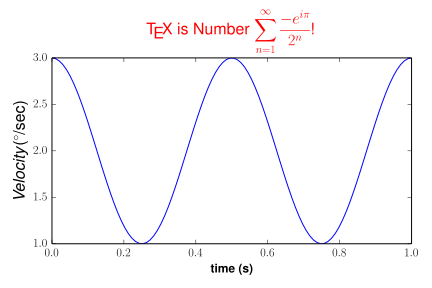
\includegraphics[width=0.7\linewidth]{dissertation-down_files/figure-latex/nice-fig-1} 

}

\caption{公式}\label{fig:nice-fig}
\end{figure}

Reference a figure by its code chunk label with the \texttt{fig:}
prefix, e.g., see Figure \ref{fig:nice-fig}. Similarly, you can
reference tables generated from \texttt{knitr::kable()}, e.g., see Table
\ref{tab:nice-tab}.

\begin{verbatim}
knitr::kable(
  head(iris, 20), caption = 'Here is a nice table!',
  booktabs = TRUE
)
\end{verbatim}

\begin{table}

\caption{\label{tab:nice-tab}Here is a nice table!}
\centering
\begin{tabular}[t]{rrrrl}
\toprule
Sepal.Length & Sepal.Width & Petal.Length & Petal.Width & Species\\
\midrule
5.1 & 3.5 & 1.4 & 0.2 & setosa\\
4.9 & 3.0 & 1.4 & 0.2 & setosa\\
4.7 & 3.2 & 1.3 & 0.2 & setosa\\
4.6 & 3.1 & 1.5 & 0.2 & setosa\\
5.0 & 3.6 & 1.4 & 0.2 & setosa\\
\addlinespace
5.4 & 3.9 & 1.7 & 0.4 & setosa\\
4.6 & 3.4 & 1.4 & 0.3 & setosa\\
5.0 & 3.4 & 1.5 & 0.2 & setosa\\
4.4 & 2.9 & 1.4 & 0.2 & setosa\\
4.9 & 3.1 & 1.5 & 0.1 & setosa\\
\addlinespace
5.4 & 3.7 & 1.5 & 0.2 & setosa\\
4.8 & 3.4 & 1.6 & 0.2 & setosa\\
4.8 & 3.0 & 1.4 & 0.1 & setosa\\
4.3 & 3.0 & 1.1 & 0.1 & setosa\\
5.8 & 4.0 & 1.2 & 0.2 & setosa\\
\addlinespace
5.7 & 4.4 & 1.5 & 0.4 & setosa\\
5.4 & 3.9 & 1.3 & 0.4 & setosa\\
5.1 & 3.5 & 1.4 & 0.3 & setosa\\
5.7 & 3.8 & 1.7 & 0.3 & setosa\\
5.1 & 3.8 & 1.5 & 0.3 & setosa\\
\bottomrule
\end{tabular}
\end{table}

You can write citations, too. For example, we are using the
\textbf{bookdown} package \citep{R-bookdown} in this sample book, which
was built on top of R Markdown and \textbf{knitr} \citep{xie2015}.

\bibliography{book.bib,packages.bib}
\addcontentsline{toc}{chapter}{\bibname}

\backmatter

\end{document}
